\section{Interface}
\subsection{Top-Level Module Interface (\texttt{Cubic\_Solver})}
The \texttt{Cubic\_Solver} module acts as the system wrapper. It accepts four FP32 coefficients representing the cubic equation $ax^3 + bx^2 + cx + d = 0$ and computes up to three complex roots formatted in coordinate form ($x\_re + j \cdot x\_im$). The control flow is governed by a standard handshake mechanism consisting of \texttt{start} and \texttt{done} signals.

\begin{figure}[H]
    \centering
    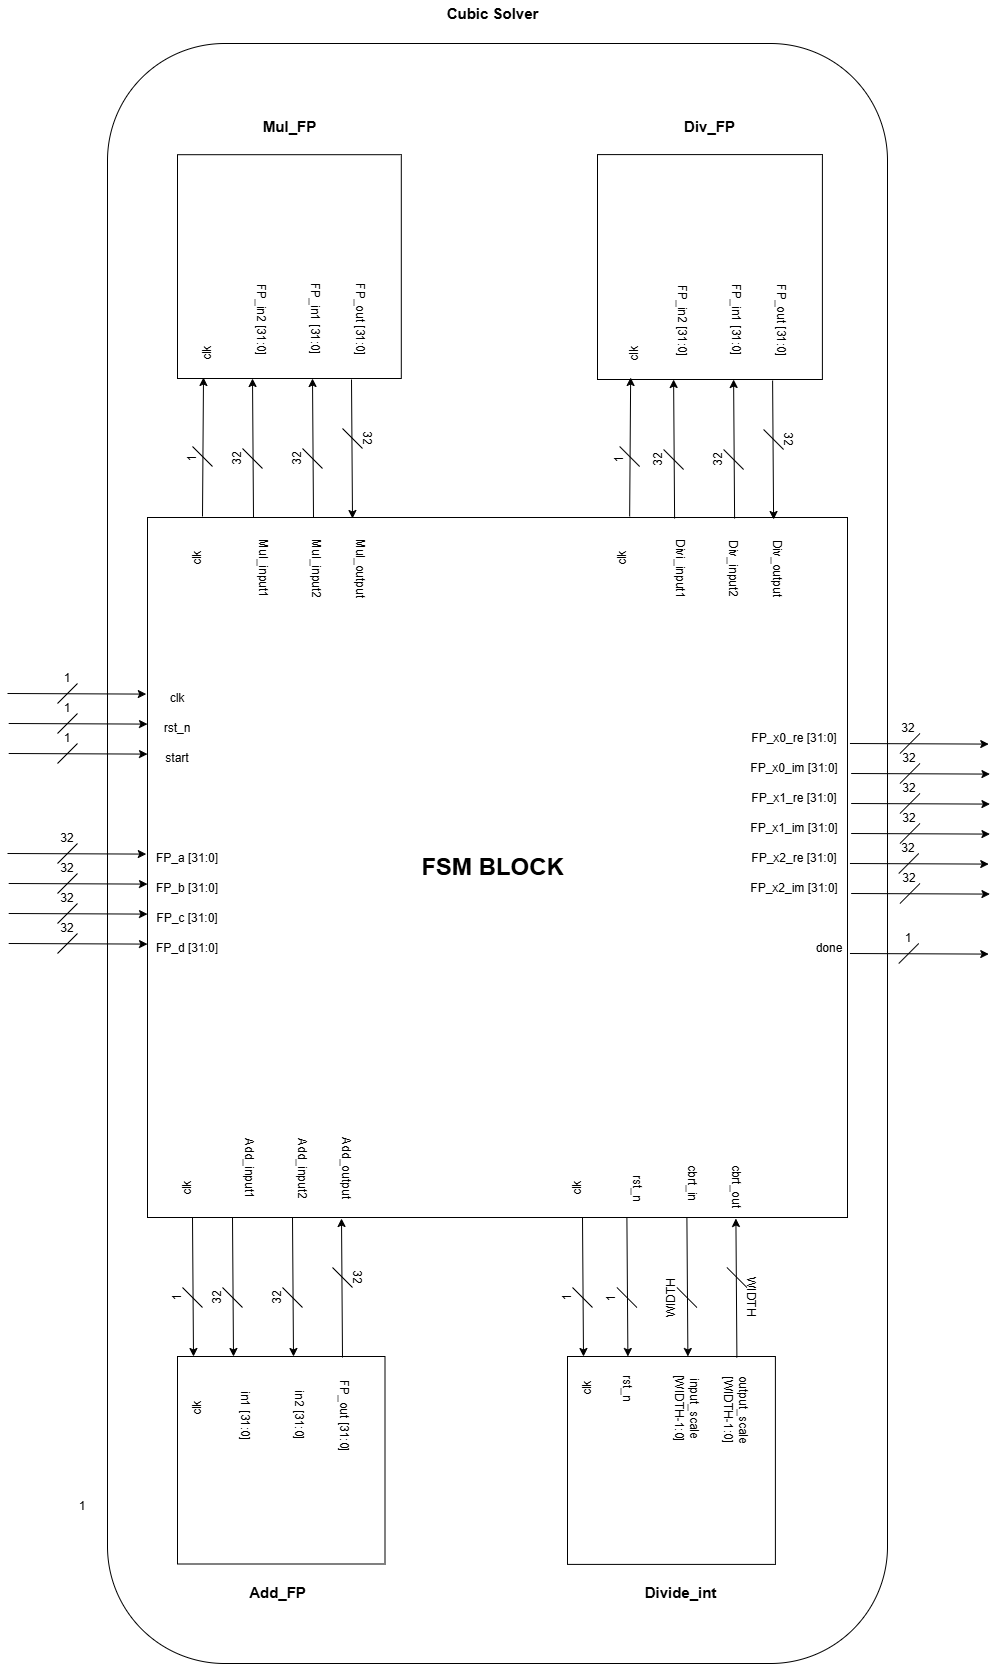
\includegraphics[width=0.6\textwidth]{graphics/cubic_solver.png}
    \caption{Top-Level Block Diagram and Interface of the Cubic Solver Module}
    \label{fig:cubic_solver_interface}
\end{figure}

The physical and logical boundary of this top-level module is defined by the following signaling groups:
\begin{itemize}
    \item [\texttt{clk} (Input, 1-bit):] Global system clock, driving all internal finite state machines (FSM) and pipeline registers on its positive edge.
    \item [\texttt{rst\_n} (Input, 1-bit):] Active-low asynchronous reset, forcing the control logic back to the \texttt{IDLE} state and clearing intermediate data registers.
    \item[\texttt{start} (Input, 1-bit):] Synchronous control pulse that triggers the FSM execution sequence. Must be asserted for at least one clock cycle to latch the input coefficients.
    \item[\texttt{FP\_a, FP\_b, FP\_c, FP\_d} (Inputs, 32-bit Bus):] Single-precision floating-point ports assigned to input the cubic equation coefficients $a, b, c,$ and $d$ respectively.
    \item[\texttt{done} (Output, 1-bit):] Handshake termination flag. Asserted high for exactly one clock cycle when the final root calculation stage is complete and valid data is locked on the outputs.
    \item[\texttt{FP\_x0\_re, FP\_x1\_re, FP\_x2\_re} (Outputs, 32-bit Bus):] Ports dedicated to outputting the real parts ($\text{Real}[x_n]$) of the three calculated roots in standard IEEE 754 single-precision format.
    \item[\texttt{FP\_x0\_im, FP\_x1\_im, FP\_x2\_im} (Outputs, 32-bit Bus):] Ports dedicated to outputting the imaginary parts ($\text{Imag}[x_n]$) of the three roots. For purely real roots, these outputs drive a static $32'h0000\_0000$ vector.
\end{itemize}

\subsection{Signed Integer Divider Interface (\texttt{Divide\_int})}
The \texttt{Divide\_int} module is a dedicated arithmetic component designed to handle signed 8-bit integer division. Within the \texttt{Cubic\_Solver} architecture, this module is specifically utilized to scale the exponents of floating-point numbers during the cube root calculation phase ($cbrt$). It operates purely on signed exponents to determine the proper scaling factor before normalization.

\begin{figure}[H]
    \centering
    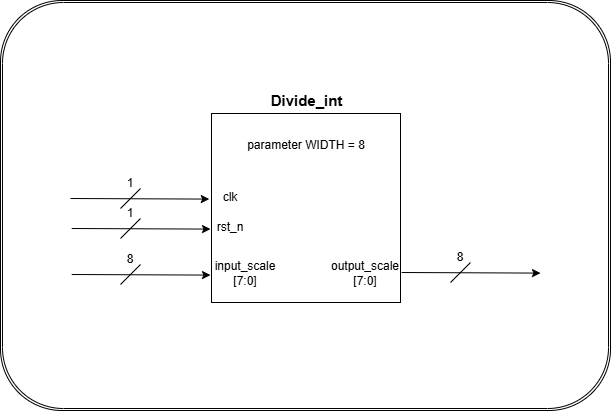
\includegraphics[width=0.5\textwidth]{graphics/div_int.png}
    \caption{Port Interface of the Signed Integer Exponent Divider Module}
    \label{fig:divide_int_interface}
\end{figure}

The hardware boundary of this helper block is defined as a purely arithmetic combinational module with the following ports:
\begin{itemize}
    \item[\texttt{input\_scale} (Input, 8-bit Bus):] Two's complement signed 8-bit integer vector carrying the raw, unadjusted exponent bias derived from the intermediate radical components.
    \item[\texttt{output\_scale} (Output, 8-bit Bus):] Two's complement signed 8-bit integer vector containing the mathematically scaled quotient value, passed directly back to the exponent adjustment logic of the cube-root normalization step.
\end{itemize}

\subsection{Floating-Point Divider Interface (\texttt{Div\_FP})}
The \texttt{Div\_FP} module implements a 16-cycle pipelined division using a Radix-4 algorithm. It comprises an input register stage, 14 iterative pipeline stages generating 2 quotient bits per cycle, and a final rounding and packing combinational unit.

\begin{figure}[H]
    \centering
    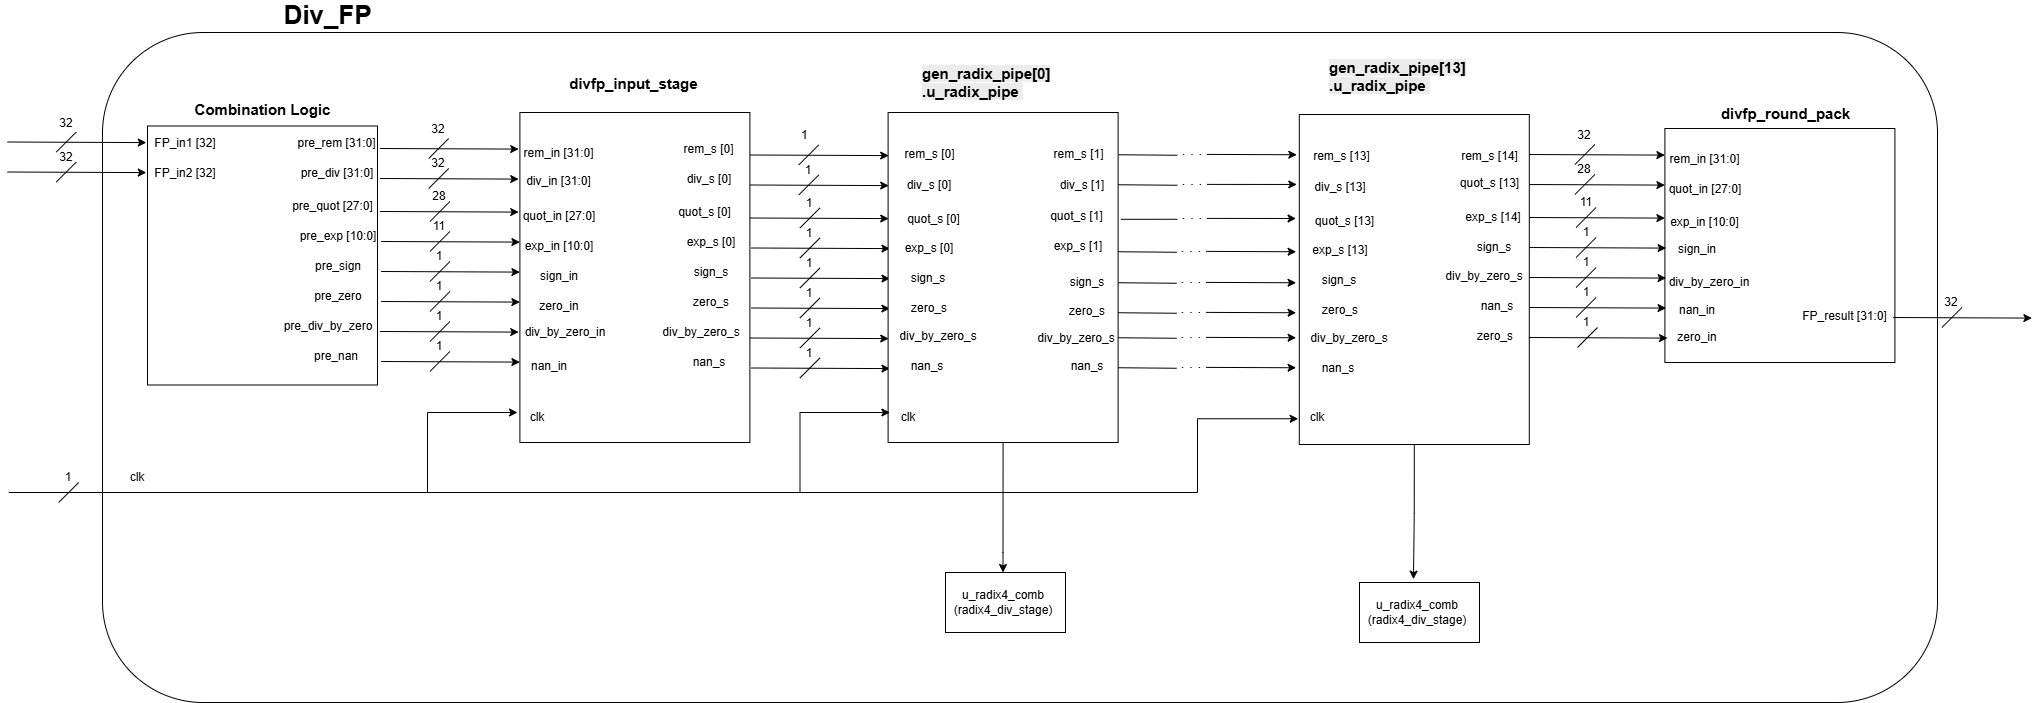
\includegraphics[width=0.9\textwidth]{graphics/div_FP.png}
    \caption{Internal Pipeline Architecture and Port Interfaces of \texttt{Div\_FP}}
    \label{fig:div_fp_interface}
\end{figure}

The macro signaling interface of the division datapath interacts via the following dedicated terminals:
\begin{itemize}
    \item[\texttt{clk} (Input, 1-bit):] Dedicated clock input running synchronously with the main system clock to toggle the 14 internal pipeline stage barriers (\texttt{gen\_radix\_pipe[0]} through \texttt{[13]}).
    \item[\texttt{FP\_in1} (Input, 32-bit Bus):] Single-precision floating-point input representing the dividend ($A$) vector.
    \item[\texttt{FP\_in2} (Input, 32-bit Bus):] Single-precision floating-point input representing the divisor ($B$) vector.
    \item[\texttt{FP\_out} (Output, 32-bit Bus):] Pipelined output port that delivers the stabilized, normalized, and rounded single-precision quotient result vector ($A/B$) after a deterministic execution latency of 16 clock cycles.
\end{itemize}

\subsection{Floating-Point Multiplier Interface (\texttt{Mul\_FP})}
The \texttt{Mul\_FP} module performs single-precision multiplication using a multi-stage architecture. It encapsulates the \texttt{MFP\_Mul} core module, which hosts a 6-stage partial product accumulation pipeline utilizing \texttt{Mul24x4} arithmetic array sub-blocks, and the \texttt{MFP\_Norm\_Rounding} unit for normalization.

\subsubsection{Module-Level External Interface}
This sub-section defines the top-level boundary of the \texttt{Mul\_FP} module. It handles the external handshaking and the raw FP32 data vectors before passing them to the internal execution cores.

\begin{figure}[H]
    \centering
    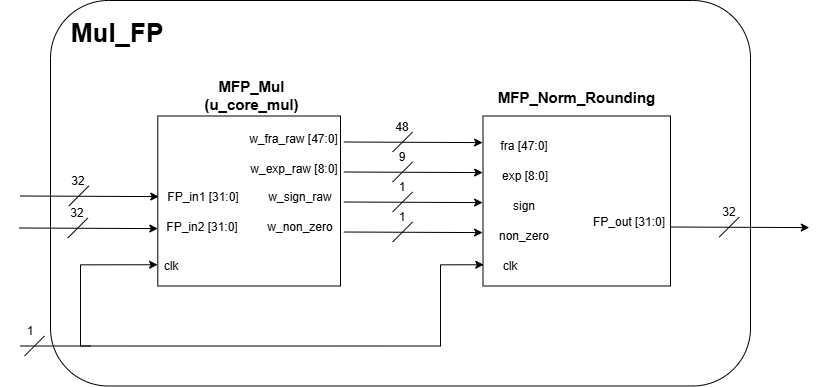
\includegraphics[width=0.7\textwidth]{graphics/mul_FP.png}
    \caption{Detailed Datapath and Port Interconnections of the Pipelined Multiplier \texttt{Mul\_FP}}
    \label{fig:mul_fp_interface}
\end{figure}

The physical external wrapper of the multi-cycle multiplier consists of the following standard ports:
\begin{itemize}
    \item[\texttt{clk} (Input, 1-bit):] Main clock connection used to advance the hidden pipeline arrays inside both the multiplication matrix and the output rounding register stage.
    \item[\texttt{FP\_in1} (Input, 32-bit Bus):] FP32 multiplicand operand input vector ($A$).
    \item[\texttt{FP\_in2} (Input, 32-bit Bus):] FP32 multiplier operand input vector ($B$).
    \item[\texttt{FP\_out} (Output, 32-bit Bus):] Standardized 32-bit IEEE 754 product result vector ($A \times B$) exposed to the central system bus.
\end{itemize}

\subsubsection{Internal Partial Product Shift-and-Add Interface}
Within the \texttt{MFP\_Mul} core, the intermediate accumulation stages (\texttt{Stage 1} through \texttt{Stage 5}) implement a hardware-optimized shift-and-add architecture. Instead of shifting the newly generated 28-bit partial product ($prod[i]$) to the left, the design shifts the previously accumulated sum ($buf\_stage_{i}$) to the right by 4 bits before feeding it into a dedicated fixed-point adder. The lower 4 bits of the old accumulator bypass the adder entirely and are directly concatenated back to form the updated bit-extended product, significantly minimizing critical path delay and saving hardware routing resources.

\begin{figure}[H]
    \centering
    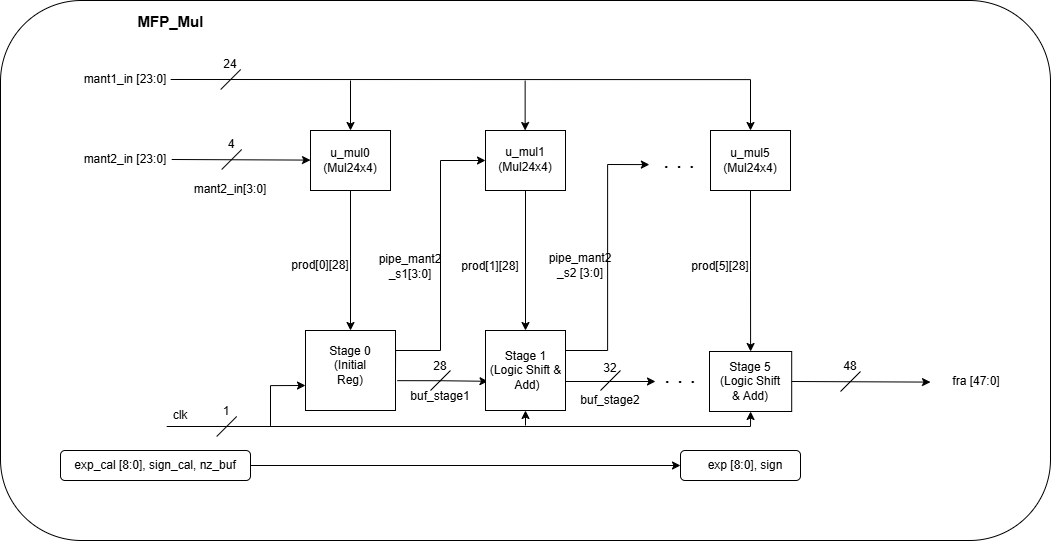
\includegraphics[width=0.8\textwidth]{graphics/MFP_mul_core.png}
    \caption{Detailed Internal Datapath of the Shift-and-Add Mechanism inside Pipeline Stages}
    \label{fig:shift_and_add_logic}
\end{figure}

The data interaction traversing the sub-boundaries of the sequential pipeline stages is formalized as follows:
\begin{itemize}
    \item[\texttt{prod[i]} (Internal Input, 28-bit Bus):] The localized static 28-bit product coming from the combinatorial \texttt{Mul24x4} array block, computed by multiplying the full 24-bit mantissa of operand $A$ with a specific 4-bit slice of operand $B$'s mantissa.
    \item[\texttt{buf\_stage\_in} (Internal Input, Variable Width):] The accumulated product bus received from the preceding stage's output register. This bus grows incrementally by 4 bits at each stage step (starting from 28 bits at \texttt{Stage 0} up to 44 bits when entering \texttt{Stage 5}).
    \item[\texttt{pipe\_mant2\_in} (Internal Input, Variable Width):] The unconsumed, remaining higher-order bits of operand $B$'s mantissa vector, shrinking by 4 bits per clock cycle as it slides through the pipeline.
    \item[\texttt{buf\_stage\_out} (Internal Output, Variable Width):] The newly calculated, bit-extended product sum captured by the localized stage register on the rising edge of the clock.
    \item[\texttt{pipe\_mant2\_out} (Internal Output, Variable Width):] The truncated multiplier $B$ vector, shifted right by 4 bits to prepare the next localized 4-bit nibble for the subsequent stage's arithmetic block.
\end{itemize}

\subsubsection{Normalization and Rounding Interface (\texttt{MFP\_Norm\_Rounding})}
After the 6-stage accumulation pipeline generates the raw 48-bit product, the datapath invokes the \texttt{MFP\_Norm\_Rounding} module. This final stage is responsible for adjusting the temporary exponent based on overflow detection, rounding the mantissa to fit the standard 23-bit width, and checking boundaries for underflow or overflow conditions.

\begin{figure}[H]
    \centering
    \includegraphics[width=0.65\textwidth]{graphics/MFP_norm_rounding.png}
    \caption{Detailed Internal Datapath of the Normalization and Rounding Mechanism}
    \label{fig:norm_rounding_logic}
\end{figure}

The sub-module interface of this normalization engine processes the following local connections:
\begin{itemize}
    \item[\texttt{w\_fra\_raw} (Internal Input, 48-bit Bus):] The final un-normalized, raw 48-bit product vector originating from the output registers of \texttt{Stage 5}.
    \item[\texttt{w\_exp\_raw} (Internal Input, 9-bit Bus):] The 9-bit unadjusted exponent sum vector calculated concurrently via the localized add operation ($E_a + E_b - 127$).
    \item[\texttt{w\_sign\_raw} (Internal Input, 1-bit):] The product parity flag bit derived from the structural asynchronous operation $S_a \oplus S_b$.
    \item[\texttt{w\_non\_zero} (Internal Input, 1-bit):] A structural zero-bypass status bit indicating whether the incoming floating-point operands are nonzero values.
\end{itemize}

\subsection{Floating-Point Adder/Subtractor Interface (\texttt{Add\_FP})}
The \texttt{Add\_FP} core executes floating-point addition and subtraction wrapped inside a 5-stage pipeline macro. The internal datapath splits the processing into sequential steps: exponent comparison (\texttt{u\_stage1}), mantissa alignment shifting (\texttt{u\_stage2}), fixed-point additions (\texttt{u\_stage3}), leading-one normalization detection (\texttt{u\_stage4}), and post-computation rounding (\texttt{u\_stage5}).

\begin{figure}[H]
    \centering
    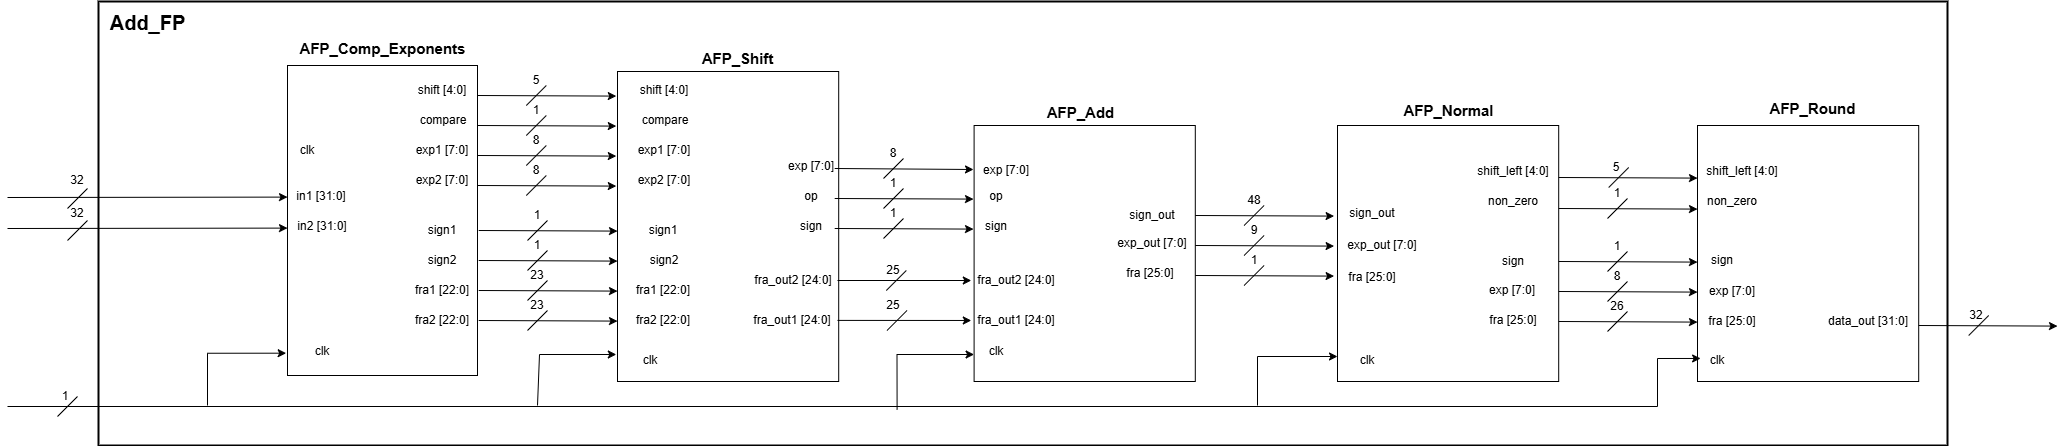
\includegraphics[width=0.7\textwidth]{graphics/add_FP.png}
    \caption{Structural Sub-module Interconnections and Interface of \texttt{Add\_FP}}
    \label{fig:add_fp_interface}
\end{figure}

The I/O interface pins bound to this algebraic calculation core are specified below:
\begin{itemize}
    \item[\texttt{clk} (Input, 1-bit):] Main clock line driving the synchronous state boundaries of the 5 internal pipeline processing blocks (\texttt{u\_stage1} through \texttt{u\_stage5}).
    \item[\texttt{in1} (Input, 32-bit Bus):] FP32 vector acting as the augend during addition operations or the minuend during subtraction operations.
    \item[\texttt{in2} (Input, 32-bit Bus):] FP32 vector acting as the addend during addition operations or the subtrahend during subtraction operations.
    \item[\texttt{data\_out} (Output, 32-bit Bus):] Stabilized 32-bit IEEE 754 single-precision sum or difference result vector, available exactly 5 clock cycles after the corresponding operands are loaded into the first stage.
\end{itemize}